\vspace*{\fill}
\begin{center}
    {\color{Black} \rule{\linewidth}{1.2mm} }\\
\vspace{0.25in}
{\centering\fontsize{30}{40}{\bfseries{\color{Black}{\scshape{Chapter V : Methodology}}}}}
\vspace{0.35in}\\
    {\color{Black} \rule{\linewidth}{1.2mm} }
\end{center}
\vspace*{\fill}
\addcontentsline{toc}{chapter}{\color{Black}{Chapter V : Methodology}}
\setcounter{section}{0}

\newpage

\section{Introduction}
\vspace{0.2in}
\hspace{\parindent}
As part of our research, we have treated the case of segmenting and counting Red, White blood cells and platelets which also known as CBC (Complete Blood Count), we are using the ALL-IDB\textsuperscript{\cite{pm77-2n23-20}} Dataset to train and evaluate our models.
In our case study, and from multiple articles, we can see that U-Net and Segnet models are dominating the field of cell segmentation and Medical Computer vision in general.
In this chapter, we test out both U-Net and Segnet models, and analyse the results by comparing results of the two architectures.
We will also explore different machine learning algorithms for both preprocessing and postprocessing.

\section{Our approach}
\vspace{0.2in}
\hspace{\parindent}
From all of the intel we have gathered, and previously read articles, all of cell segmentation (blood cell segmentation in particular) are mostly using U-Net and Segnet archtectures for segmenting blood cell images.
We have implemented both the U-Net and Segnet models.
In the following sections, we will briefly analyze and compare both convolutional neural network (CNN) models with their perspective results.
And explain all the postprocessing methods we used for the counting of blood cells (red, white and platelets)

\section{DO-UNet}
\subsection{Definition}
\hspace{\parindent}
The U-Net is a convolutional neural network that was developed for biomedical image segmentation at the Computer Science Department of the University of Freiburg. The network is based on the fully convolutional network and its architecture was modified and extended to work with fewer training images and to yield more precise segmentations. In our case we are using DO-UNet from \textsuperscript{\cite{10.1007/978-3-030-44584-3_31}} which is a modified U-Net to produce dual outputs, which also known as contour aware network was first demonstrated by the DCAN architecture \textsuperscript{\cite{chen2016dcan}}.  Based on a simple FCN, DCAN was trained to use the outer
contours of the areas of interest to guide the training of the segmentation masks. This led to improved semantic and instance segmentation of the model, which in their case, looked at non-overlapping features in biomedical imaging.
With the aim of counting closely co-located and overlapping cells, we are predominantly interested in the correct detection of individual objects as
opposed to the exact precision of the segmentation mask itself. An examination
of the hidden convolutional layers of the classical U-Net showed that the penultimate layer of the network extracts information about the edges of the cells, so the idea is to output the cell mask + edge mask then do a substraction to break the overlapping cells.

\subsection{Architecture}
\hspace{\parindent}
They Started with the classical U-Net then reduced the number of
convolutional layers and skip connections in the model. Simultaneously, they minimised the complexity of the model by looking at smaller input regions of the images, thus minimising the memory footprint of the model. They follow the approach of Ronneberger et. al. \textsuperscript{\cite{10.1007/978-3-030-44584-3_31}} by using unpadded convolutions throughout the network, resulting in a model with smaller output edge and mask (100 × 100 px) corresponding to a central region of a larger (188 × 188 px) input image region. DO-U-Net uses two, independently trained, output layers of identical size. Figure \ref{fig:DO-UNET} shows the DO-U-Net architecture.

\begin{figure}[H]
\centering
  \vspace{-0.1in}
    \centerline{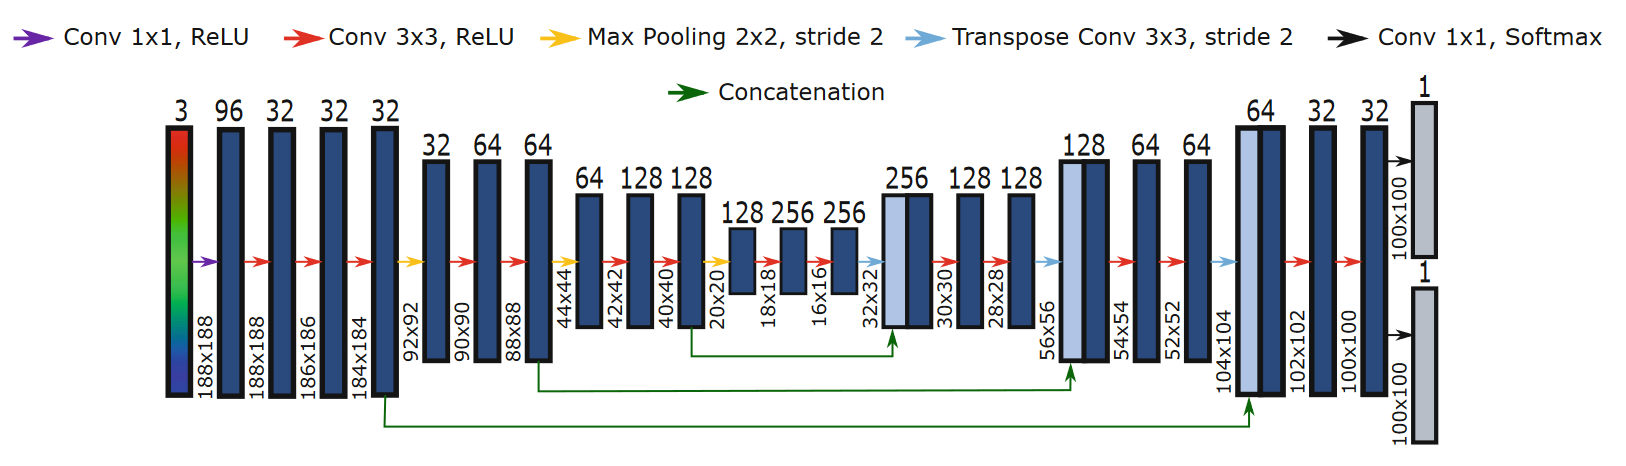
\includegraphics[width = \linewidth]{../images/DO-UNET.png}}
    \caption{DO-UNet architecture}
    \label{fig:DO-UNET}
\end{figure}

\section{Segnet}
\subsection{Definition}
\hspace{\parindent}
The SegNet neural network, developed by Alex Kendall, Vijay Badrinarayanan, and Roberto Cipolla, all from the University of Cambridge, is a convolutional neural network used for semantic pixel wise labeling. This problem is more commonly called semantic segmentation. \textsuperscript{\cite{badrinarayanan2017segnet}}

\subsection{Architecture}
\hspace{\parindent}
SegNet has an encoder network and a corresponding decoder network, followed by a final pixelwise classification layer. This architecture is illustrated in the below figure.
With 13 encoder layers obtained from the VGG16 network, and 13 decoder layers to match the same number of encoder layers. The final decoder output is fed to a multi-class soft-max classifier to produce class probabilities for each pixel independently (pixelwise).

Each encoder in the encoder network performs convolution with a filter bank to produce a set of feature maps. These are then batch normalized. Then an element-wise rectified- linear non-linearity (ReLU) max(0, x) is applied. Following that, max-pooling with a 2x2 window and stride 2 (non-overlapping window) is performed and the resulting output is sub-sampled by a factor of 2. Max-pooling is used to achieve translation invariance over small spatial shifts in the input image.

The appropriate decoder in the decoder network upsamples its input feature map(s) using the memorized max-pooling indices from the corresponding encoder feature map(s). This step pro- duces sparse feature map(s). This SegNet decoding technique is illustrated in the below figure.
These feature maps are then convolved with a trainable decoder filter bank to produce dense feature maps. A batch normalization step is then applied to each of these maps. Note that the decoder corresponding to the first encoder (closest to the input image) produces a multi-channel feature map, although its encoder input has 3 channels (RGB).
This is unlike the other decoders in the network which produces feature maps with the same number of size and channels as their encoder inputs. The high dimensional feature representation at the output of the final decoder is fed to a trainable soft-max classifier.
This soft-max classifies each pixel independently. The output of the soft-max classifier is a K channel image of probabilities where K is the number of classes. The predicted segmentation corresponds to the class with maximum probability at each pixel. \textsuperscript{\cite{badrinarayanan2017segnet}}

\vspace{0.2in}

\begin{figure}[H]
\centering
  \vspace{-0.1in}
    \centerline{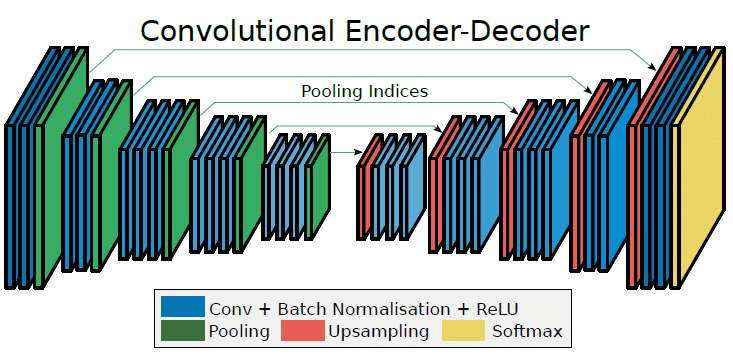
\includegraphics[width = 3.5in]{../images/segnet.png}}
    \caption{SegNet architecture}
\end{figure}

\subsection{Dataset}
\hspace{\parindent}
For the segnet model, we have decided to test the ALL-IDB1 dataset, which contains 108 blood cell images, of which 10 images with their perspective masks and edge masks were chosen for red blood cell training and 3 as a test dataset, for white blood cells 73 images with their masks, and 33 as a test dataset.
For platelets, we used 71 for training and 31 as a test dataset.
Only red blood cells have edge masks, because we need to get rid of overlapped cells, white blood cells and platelets dont need the edge masks, using masks only can retrieve all the necessary features, because both white blood cells and platelets rarely overlap.
The images will be sliced and rescaled to 128x128 to match the input shape of the Segnet model.
The resulting train dataset will be 3916 image, mask, and edge tiles (a total of 11748 tiles).
For the test dataset 1072 image, mask, and edge tiles (a total of 3216 tiles) for red blood cells.
As for white blood cells, 28126 image and mask tiles were used for training (a total of 56252 tiles), and 15892 image and mask tiles were used as a test dataset for white blood cells (a total of 31784 tiles).
Finally, for platelets we used 27650 image and mask tiles were used for training (a total of 55300), and 14410 image and mask tiles as a test dataset for platelets (a total of 28820).

\vspace{0.1in}

% Please add the following required packages to your document preamble:
% \usepackage{multirow}
% \usepackage{graphicx}
% \usepackage[table,xcdraw]{xcolor}
% If you use beamer only pass "xcolor=table" option, i.e. \documentclass[xcolor=table]{beamer}
\begin{table}[H]
\centering
\resizebox{\textwidth}{!}{%
\begin{tabular}{|cc|c|c|c|c|c|c|}
\hline
\multicolumn{2}{|c|}{{\color[HTML]{000000} \textbf{Dataset}}}                                                                     & {\color[HTML]{000000} \textbf{\begin{tabular}[c]{@{}c@{}}Train\\ images\end{tabular}}} & {\color[HTML]{000000} \textbf{\begin{tabular}[c]{@{}c@{}}Test\\ images\end{tabular}}} & {\color[HTML]{000000} \textbf{\begin{tabular}[c]{@{}c@{}}Train\\ Tiles\end{tabular}}} & {\color[HTML]{000000} \textbf{\begin{tabular}[c]{@{}c@{}}Test\\ Tiles\end{tabular}}} & {\color[HTML]{000000} \textbf{\begin{tabular}[c]{@{}c@{}}Total\\ images\end{tabular}}} & {\color[HTML]{000000} \textbf{\begin{tabular}[c]{@{}c@{}}Total\\ tiles\end{tabular}}} \\ \hline
\multicolumn{1}{|c|}{{\color[HTML]{000000} }}                                             & {\color[HTML]{000000} \textbf{Image}} & {\color[HTML]{000000} 10}                                                              & {\color[HTML]{000000} 3}                                                              & {\color[HTML]{000000} 3916}                                                           & {\color[HTML]{000000} 1072}                                                          & {\color[HTML]{000000} 13}                                                              & {\color[HTML]{000000} \textbf{4988}}                                                  \\ \cline{2-8} 
\multicolumn{1}{|c|}{{\color[HTML]{000000} }}                                             & {\color[HTML]{000000} \textbf{Mask}}  & {\color[HTML]{000000} 10}                                                              & {\color[HTML]{000000} 3}                                                              & {\color[HTML]{000000} 3916}                                                           & {\color[HTML]{000000} 1072}                                                          & {\color[HTML]{000000} 13}                                                              & {\color[HTML]{000000} \textbf{4988}}                                                  \\ \cline{2-8} 
\multicolumn{1}{|c|}{\multirow{-3}{*}{{\color[HTML]{000000} \textbf{Red Blood Cells}}}}   & {\color[HTML]{000000} \textbf{Edge}}  & {\color[HTML]{000000} 10}                                                              & {\color[HTML]{000000} 3}                                                              & {\color[HTML]{000000} 3916}                                                           & {\color[HTML]{000000} 1072}                                                          & {\color[HTML]{000000} 13}                                                              & {\color[HTML]{000000} \textbf{4988}}                                                  \\ \hline
\multicolumn{1}{|c|}{{\color[HTML]{000000} }}                                             & {\color[HTML]{000000} \textbf{Image}} & {\color[HTML]{000000} 73}                                                              & {\color[HTML]{000000} 33}                                                             & {\color[HTML]{000000} 28126}                                                          & {\color[HTML]{000000} 15892}                                                         & {\color[HTML]{000000} 106}                                                             & {\color[HTML]{000000} \textbf{44018}}                                                 \\ \cline{2-8} 
\multicolumn{1}{|c|}{\multirow{-2}{*}{{\color[HTML]{000000} \textbf{White Blood Cells}}}} & {\color[HTML]{000000} \textbf{Mask}}  & {\color[HTML]{000000} 73}                                                              & {\color[HTML]{000000} 33}                                                             & {\color[HTML]{000000} 28126}                                                          & {\color[HTML]{000000} 15892}                                                         & {\color[HTML]{000000} 106}                                                             & {\color[HTML]{000000} \textbf{44018}}                                                 \\ \hline
\multicolumn{1}{|c|}{{\color[HTML]{000000} }}                                             & {\color[HTML]{000000} \textbf{Image}} & {\color[HTML]{000000} 71}                                                              & {\color[HTML]{000000} 31}                                                             & {\color[HTML]{000000} 27650}                                                          & {\color[HTML]{000000} 14410}                                                         & {\color[HTML]{000000} 102}                                                             & {\color[HTML]{000000} \textbf{42060}}                                                 \\ \cline{2-8} 
\multicolumn{1}{|c|}{\multirow{-2}{*}{{\color[HTML]{000000} \textbf{Platelets}}}}         & {\color[HTML]{000000} \textbf{Mask}}  & {\color[HTML]{000000} 71}                                                              & {\color[HTML]{000000} 31}                                                             & {\color[HTML]{000000} 27650}                                                          & {\color[HTML]{000000} 14410}                                                         & {\color[HTML]{000000} 102}                                                             & {\color[HTML]{000000} \textbf{42060}}                                                 \\ \hline
\end{tabular}%
}
\caption{Dataset used for segnet}
\label{Dataset used for segnet}
\end{table}


\section{Dataset augmentation}
\hspace{\parindent}
We used the same dataset augmention on all cells (red, white blood cells, and platelets) in both models UNet and SegNet.
The augmentation we used was custom which involves the following steps:
\begin{enumerate}
    \item Pick a random image from the train dataset.
    \item Get the x and y coordinates randomly from the chosen image.
    \item Rescale the image randomly to a smaller size then scale it back to the original size to reduce quality.
    \item Take a slice of the image and mask accordingly and also edge if available.
    \item Skip the image if it dosn't contain out object of interest
    \item Resize the image and mask to the model input.
    \item Randomly rotate and flip the image chip.
    \item Randomly augment the colors (luminosity and saturation).
\end{enumerate}

\begin{figure}[H]
\centering
  \vspace{-0.1in}
    \centerline{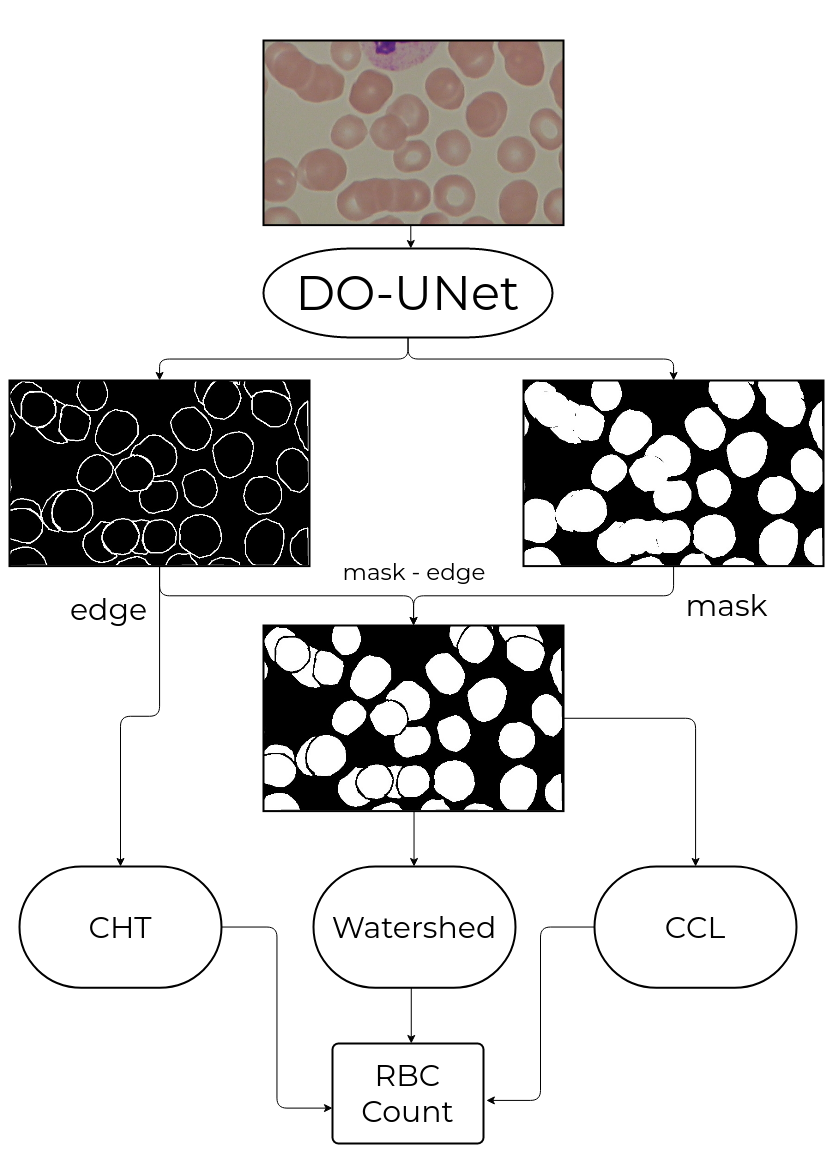
\includegraphics[width = 7in]{../images/Diag_RBC_DOUNET_SegNet.png}}
    \caption{Schema of the segmentation and counting steps of the RBC's}
    \label{fig:scheme_RBC}
\end{figure}

\begin{figure}[H]
\centering
  \vspace{-0.1in}
    \centerline{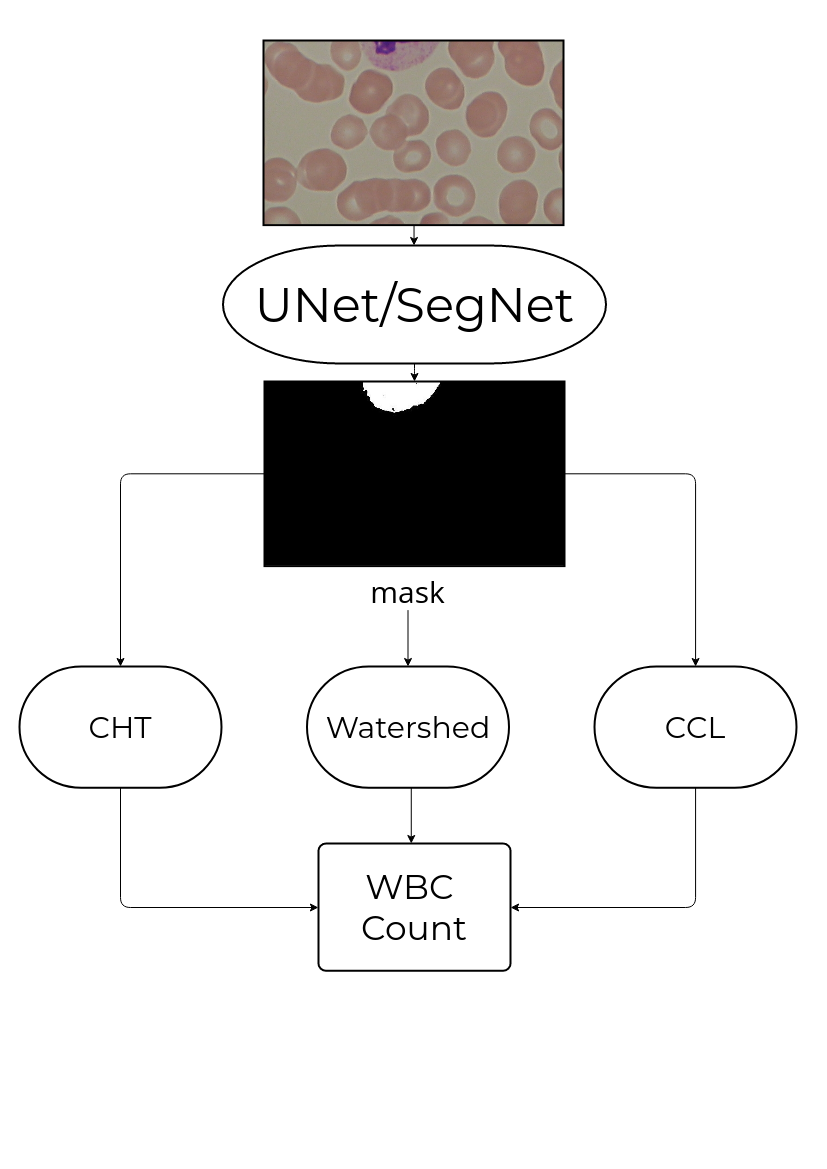
\includegraphics[width = 7in]{../images/Diag_WBC_PLT_UNET_SegNet.png}}
    \caption{Schema of the segmentation and counting steps of the WBC's and Platelets}
    \label{fig:scheme_WBC_PLT}
\end{figure}

\section{Counting}
\vspace{0.2in}
\hspace{\parindent}
After having segmented blood cell images (red, white blood cells and platelets), we use multiple post-processing methods (machine learning algorithms) to get the coordinates of circles and count them. as we can see in fig \ref{fig:scheme_RBC} and  \ref{fig:scheme_WBC_PLT}.\\
We can see below are all the algorithms we used to get an relatively accurate blood cell count:

\subsection{Circle Hough Transform}
\hspace{\parindent}
Circle Hough Transform (CHT) is machine learning algorithm used to extract features (circles) from imperfect images.
We modified its parameters (Minimum distance, Minimum and Maximum radius...) for each type of blood cells (red, white and platelets).\\
Note that we do not rely on this approach to count white blood cells, because most white blood cells have different shapes.
Therefore, this method is useless when it comes to white blood cells counting.

We Modified this method by adding a loss function which will help us to eliminate False Positives circles by calculating the percentage of the intersection between the circle and the cell mask. we improved the counting accuracy by more than 20\% with a threshold intersection percentage of 60\%.

%TODO Graph

\subsection{Connected Component Labeling}
\hspace{\parindent}
Connected Component Labeling (CCL) is machine learning algorithm used to detect connected regions in a binary image.
Before applying the connected component labeling, we convert the images to gray-scale. Then, a binary threshold is applied to the images to get binary values.
Finally, we apply the connected component labeling to get the labels and map component labels to the resulting image, and the number of labels is the cell count accordingly.

\begin{figure}[H]
\centering
\begin{minipage}{.5\textwidth}
  \centering
  \centerline{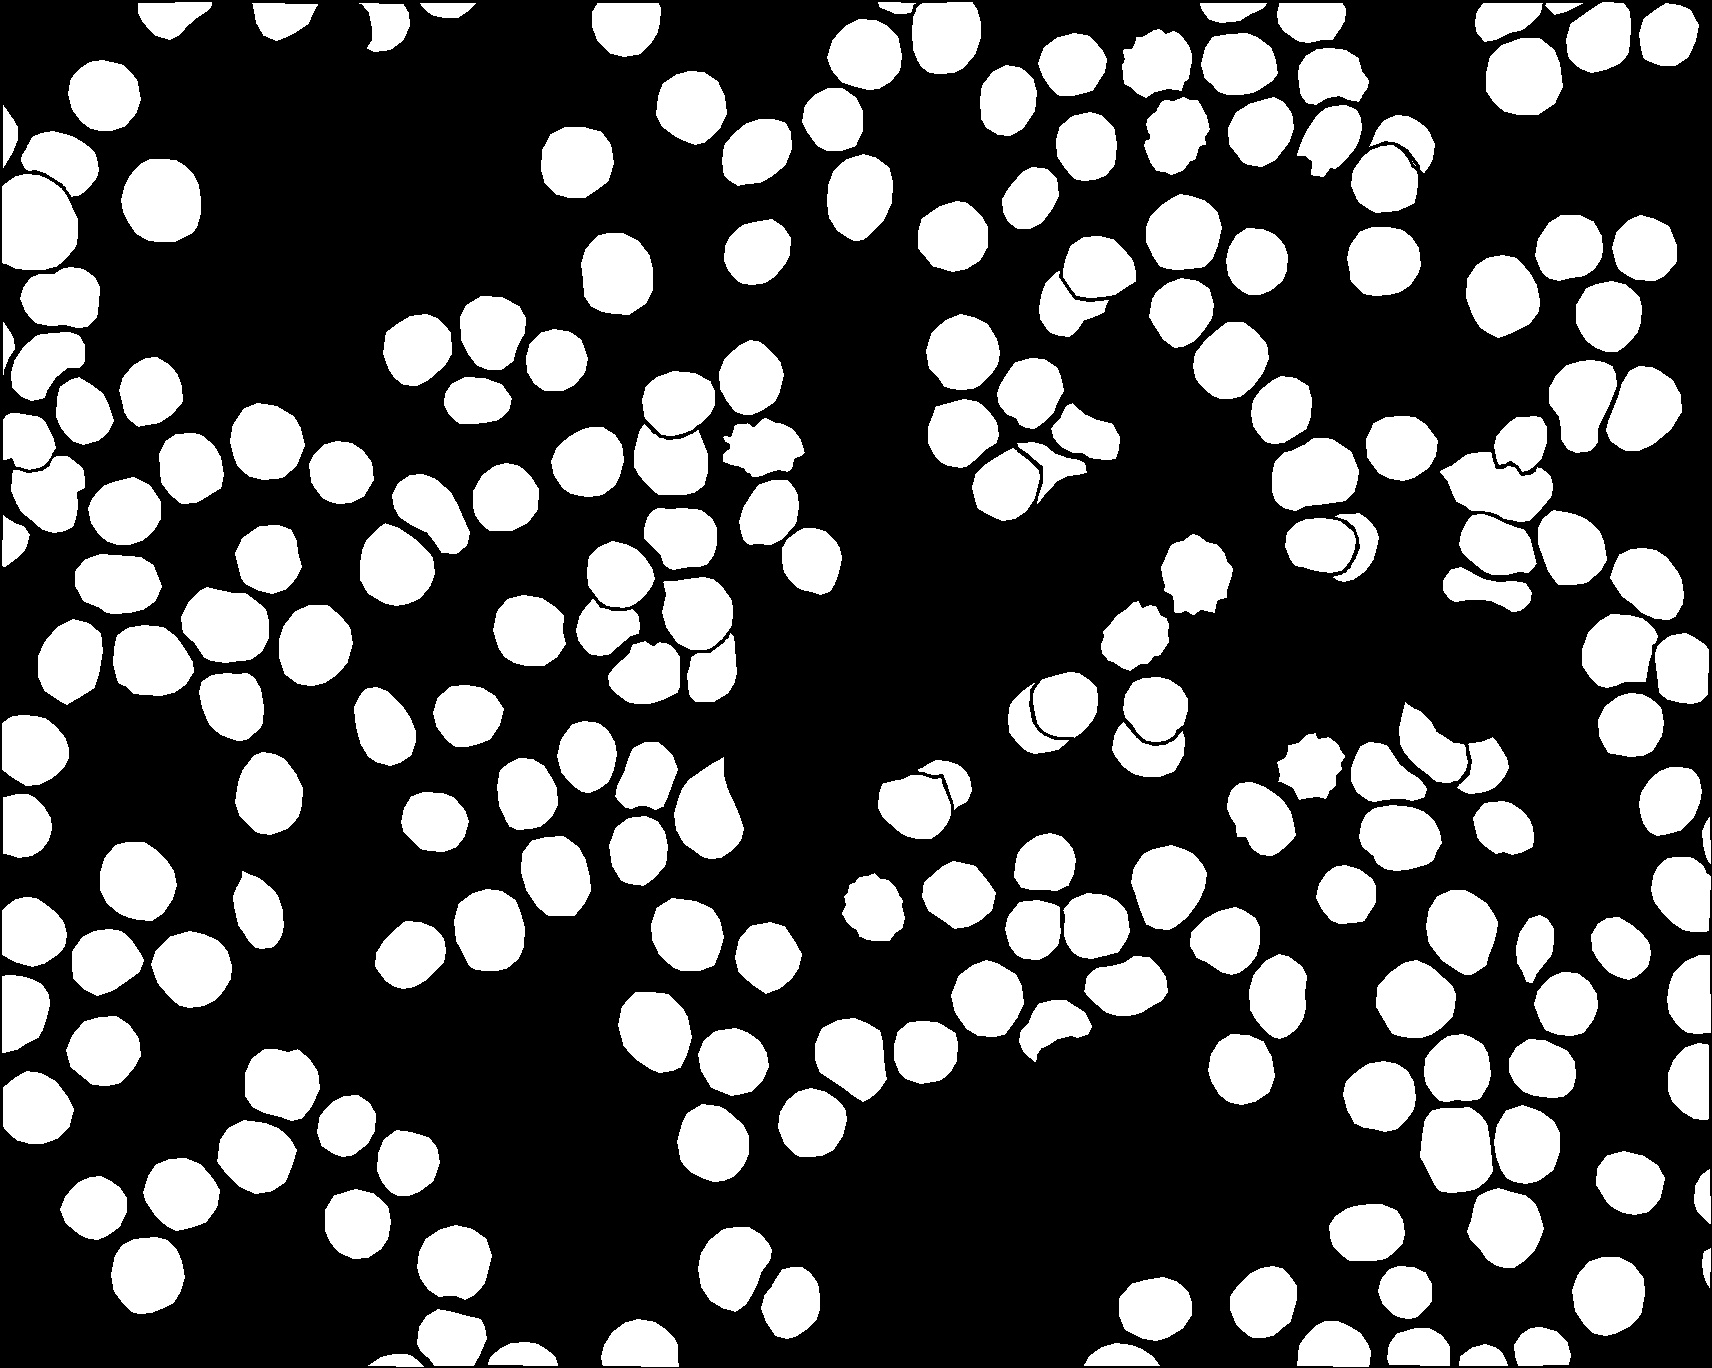
\includegraphics[width = 77mm]{../images/Im0001_1_substraction.jpg}}
    \subcaption{input Image}
\end{minipage}%
\begin{minipage}{.5\textwidth}
  \centering
  \centerline{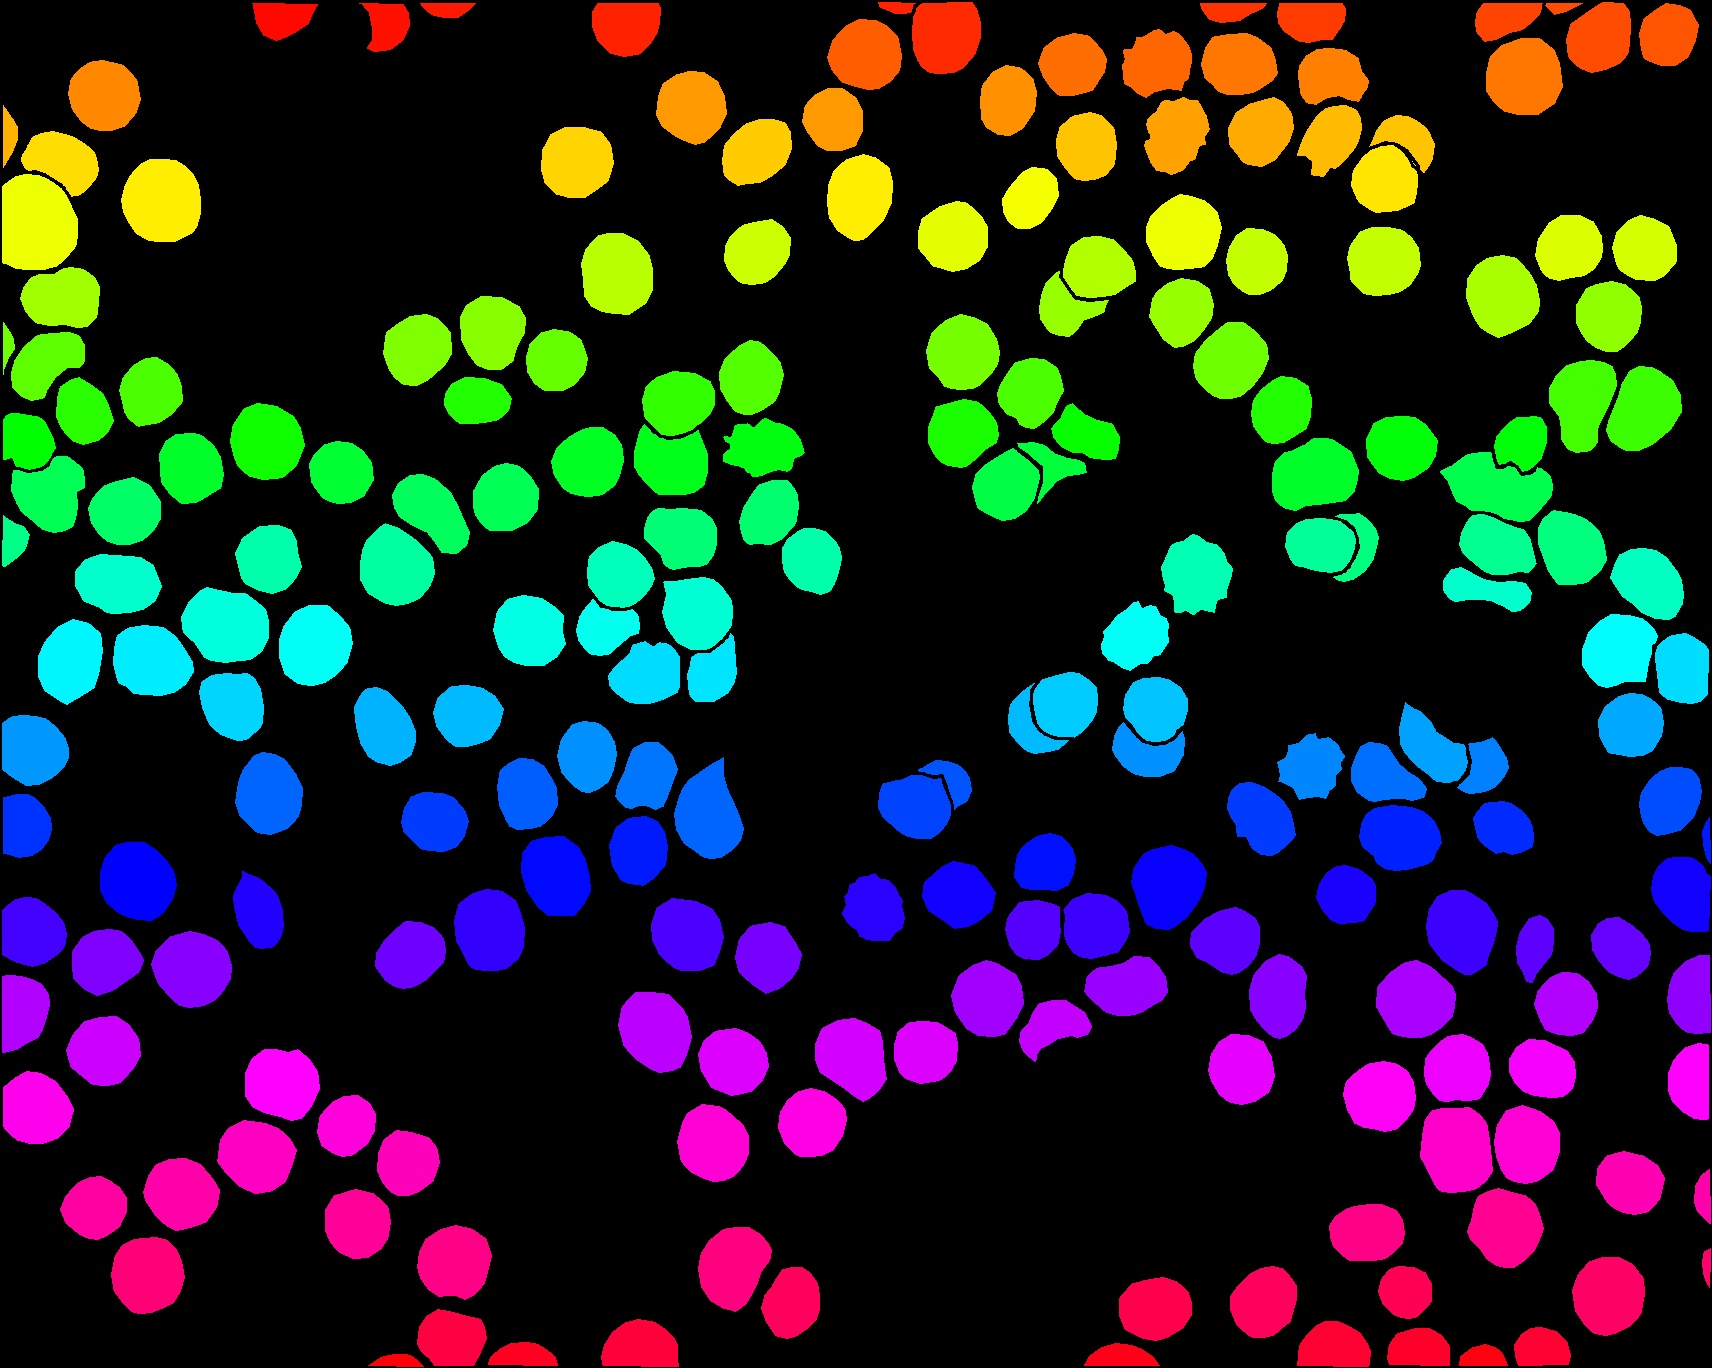
\includegraphics[width = 77mm]{../images/Im0001_1_connected_compounent_labeling.jpg}}
    \subcaption{output image}
\end{minipage}
  \caption{Example of connected component labeling}
\end{figure}

\subsection{Watershed}
\hspace{\parindent}
Watershed algorithms (also called drainage divide) are used in image processing primarily for object segmentation purposes, that is, for separating different objects in an image. the main purpose of using watershed in this phase is to segment the touching and overlapping cells, the watershed takes two inputs, first i takes an image with different intensity levels in our-case the distance transform of our mask where the intensity levels represents reliefs. the second input is the water sources in our-case we extracted local maxima from the distance transform image. we can see below the steps we used to count the cells.

\begin{enumerate}
    \item \textbf{Compute the Euclidean distance}: we compute euclidean distance from every binary pixel to the nearest zero pixel, this map will be used as our relief map in the watershed algorithm.
    \item \textbf{We find peaks in the distance map}: we search for peaks in our euclidean distance map which is the local maxima in each region, which are the highest points in the map (higher intensity levels), which we will use as water sources in the watershed algorithm.
    \item \textbf{Apply connected component labeling on the peak map}: we apply CCL algorithm which is also called 8-connectivity algorithm to label the peaks (label each water source).
    \item \textbf{Apply the Watershed algorithm on the reversed distance map using the labeled peaks}: at the end we feed the reversed distance map and the water sources map (local maxima) to the watershed algorithm to get the segmented image. 
\end{enumerate}

Here is a schema presenting the previously mentioned steps:

\begin{figure}[H]
\centering
  \vspace{-0.1in}
    \centerline{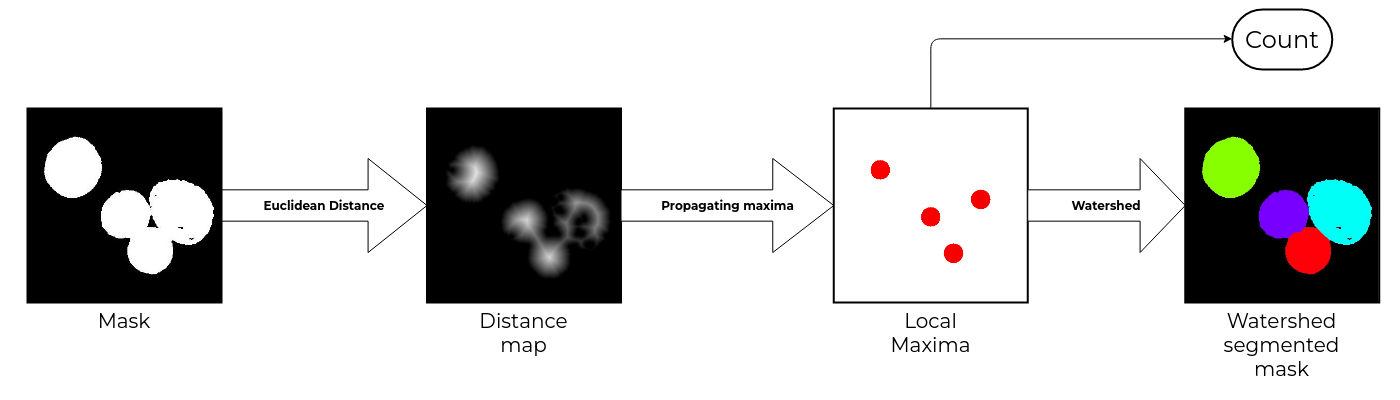
\includegraphics[width = 7in]{../images/watershed.png}}
    \caption{Watershed schema applied to count white blood cells}
\end{figure}

\section{Metrics And Loss Functions}
\hspace{\parindent}
Loss functions are one of the important ingredients in deep learning-based medical image segmentation methods. In the past four years, more than 20 loss functions have been proposed for various segmentation tasks. Most of them can be used in any segmentation tasks in a plug-and-play way, we can see in (fig \ref{fig:LossFunctions}) the relations between the most used  Loss Functions, we will present below the used Loss Functions in our paper.

\begin{figure}[H]
\centering
  \vspace{-0.1in}
    \centerline{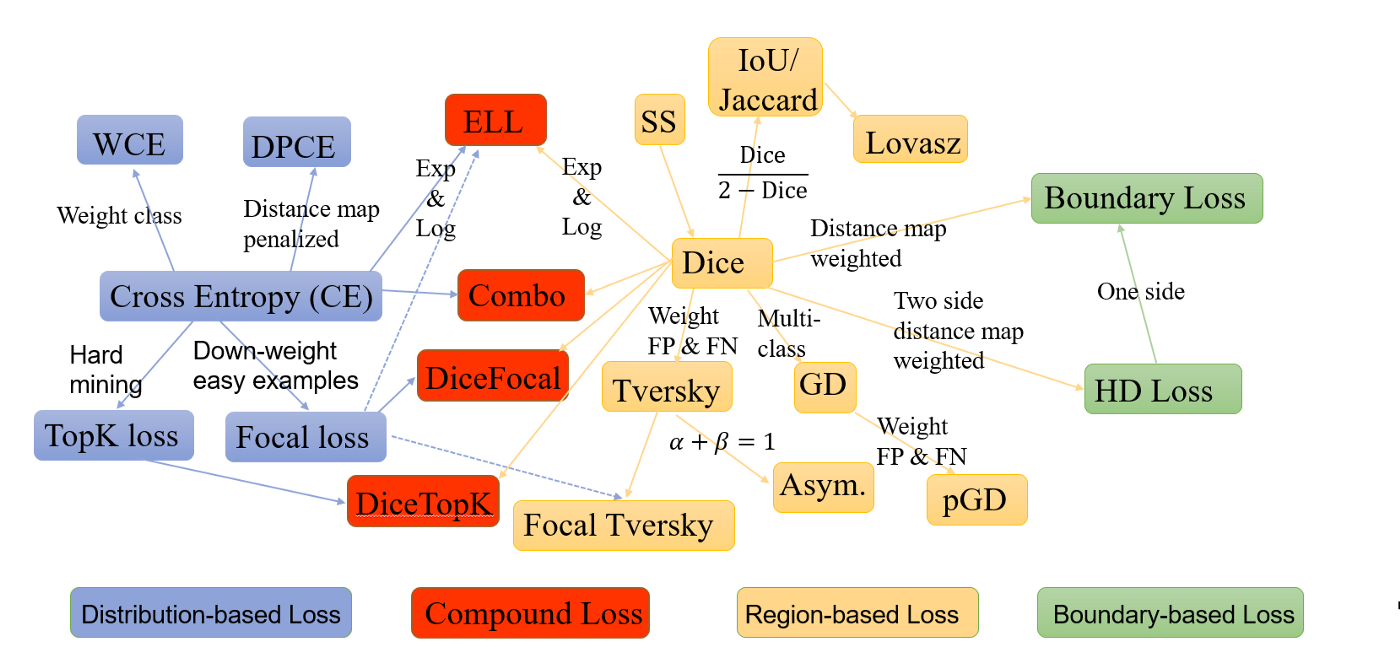
\includegraphics[width = \linewidth]{../images/LossFunctions.png}}
    \caption{Loss Functions}
    \label{fig:LossFunctions}
\end{figure}

In this section, we will discuss the loss functions and metrics that we used to train and evaluate our models.

When performing classification predictions (pixel-wise classification in our case) there's four types of outcomes that could occur.

\begin{enumerate}
    \item \textbf{True positives} are when you predict an observation belongs to a class and it actually does belong to that class.
    \item \textbf{True negatives} are when you predict an observation does not belong to a class and it actually does not belong to that class.
    \item \textbf{False positives} occur when you predict an observation belongs to a class when in reality it does not.
    \item \textbf{False negatives} occur when you predict an observation does not belong to a class when in fact it does.
\end{enumerate}

These four outcomes are often plotted on a confusion matrix. The following confusion matrix is an example for the case of binary classification. This matrix should be generated making predictions on the test data and then identifying each prediction as one of the four possible outcomes described above.

\vspace{0.1in}

\begin{table}[H]
\centering
\begin{tabular}{cc|cc|}
\cline{3-4}
\multicolumn{2}{c|}{\multirow{2}{*}{}}                                                                                        & \multicolumn{2}{c|}{\textbf{Actual Values}}             \\ \cline{3-4} 
\multicolumn{2}{c|}{}                                                                                                         & \multicolumn{1}{c|}{\textbf{Yes (1)}} & \textbf{No (0)} \\ \hline
\multicolumn{1}{|c|}{\multirow{2}{*}{\textbf{\begin{tabular}[c]{@{}c@{}}Predicted\\ Values\end{tabular}}}} & \textbf{Yes (1)} & \multicolumn{1}{c|}{\textbf{TP}}      & \textbf{FP}     \\ \cline{2-4} 
\multicolumn{1}{|c|}{}                                                                                     & \textbf{No (0)}  & \multicolumn{1}{c|}{\textbf{FN}}      & \textbf{TN}     \\ \hline
\end{tabular}
\caption{Confusion Matrix}
\label{Confusion Matrix}
\end{table}


The three main metrics used to evaluate a classification model are accuracy, precision, and recall.

Accuracy is defined as the percentage of correct predictions for the test data. It can be calculated easily by dividing the number of correct predictions by the number of total predictions.

\begin{equation}
  Accuracy = \frac{Correct\; Predictions}{All\; Predictions}
\end{equation}

Precision is defined as the fraction of relevant examples (true positives) among all of the examples which were predicted to belong in a certain class.

\begin{equation}
  Precision = \frac{True\; Positives}{True\; Positives + False\; Positives}
\end{equation}

Recall is defined as the fraction of examples which were predicted to belong to a class with respect to all of the examples that truly belong in the class.

\begin{equation}
  Recall = \frac{True\; Positives}{True\; Positives + False\; Negatives}
\end{equation}

We have a semantic segmentation problem. Therefore, we use the following metrics:

\subsection{Pixel Accuracy}
\hspace{\parindent}
Pixel accuracy is perhaps the easiest to understand conceptually. It is the percent of pixels in the input image that are classified correctly.\

We don't rely on this metric because it is susceptible to class-imbalance, which is when the classes are extremely imbalanced, it means that a class or some classes dominate the image, while some other classes make up only a small portion of the image. Unfortunately, class imbalance is prevalent in many real world data sets, so it can’t be ignored.\

To further illustrate this, if an input image was 100\% black, the output prediction would be above 90\% accurate, which is a totally false prediction as presented in the figure below.

\vspace{0.1in}

\begin{figure}[H]
\centering
  \vspace{-0.1in}
    \centerline{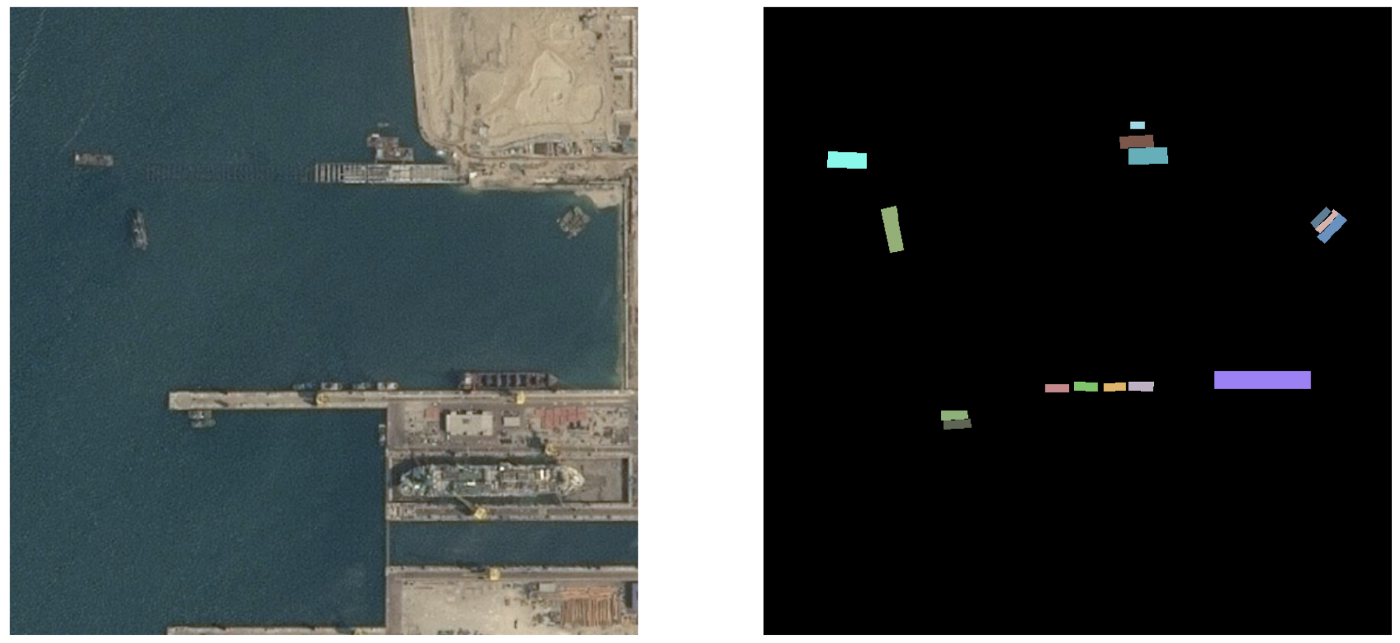
\includegraphics[width = 3.4in]{../images/class_imbalance.png}}
    \caption{Example class imbalance}
\end{figure}

\subsection{IOU}
\hspace{\parindent}
The Jaccard Index or Intersection Over Union, also known as the Jaccard similarity coefficient, is a statistic (metric) used for gauging the similarity and diversity of sample sets. It was developed by Grove Karl Gilbert in 1884 as his ratio of verification (v),\textsuperscript{\cite{murphy1996finley}} and now is frequently referred to as the Critical Success Index in meteorology. It was later developed independently by Paul Jaccard, originally giving the French name coefficient de communauté.\textsuperscript{\cite{jaccard1912distribution}} The Jaccard coefficient measures similarity between finite sample sets, and is defined as the size of the intersection divided by the size of the union of the sample sets, here is the formula:

\begin{equation}
    J(A,B) = \frac{Area\; of\; Overlap}{Area\; of\; Union} = \frac{|A \cap B|}{|A \cup B|}
\end{equation}

Here is an example of using IOU on a stop sign, where the green bounding box is the ground truth (the right prediction) and the red bounding box is what the model predicted.

\vspace{0.1in}

\begin{figure}[H]
\centering
  \vspace{-0.1in}
    \centerline{\fbox{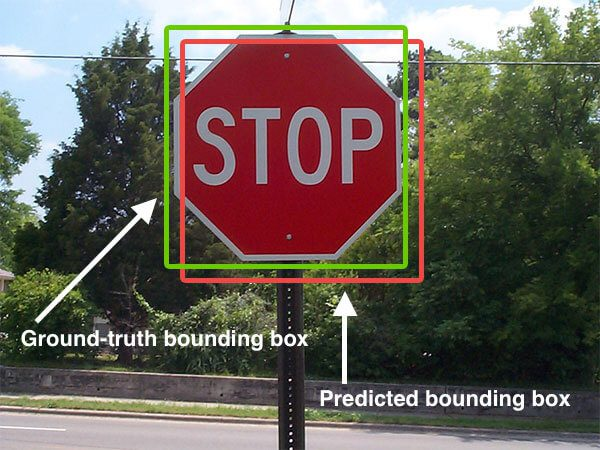
\includegraphics[width = 3.5in]{../images/exampleIOU.jpg}}}
    \caption{Example of IOU applied on a stop sign image}
\end{figure}

\subsection{Dice}
\hspace{\parindent}
The Sørensen–Dice coefficient is a statistic used to measure the similarity of two samples, It was developed by the botanists (scientific study of plants) Thorvald Sørensen and Lee Raymond Dice, who published in 1948 and 1945 respectively.\\
Sørensen's original formula was intended to be applied to discrete data. Given two sets, X and Y, it is defined as :
\begin{equation}
    DSC(X, Y) = \frac{2 | X \cap Y |}{| X |  +  | Y |}
\end{equation}
where |X| and |Y| are the cardinalities of the two sets . The Sørensen index equals twice the number of elements common to both sets divided by the sum of the number of elements in each set as we can see in fig \ref{fig:DSC_EX}. 
When applied to Boolean data, using the definition of true positive (TP), false positive (FP), and false negative (FN), it can be written as :
\begin{equation}
    DSC = \frac{2 TP}{2 TP + FN + FP}
\end{equation}

\begin{figure}[H]
\centering
  \vspace{-0.1in}
    \centerline{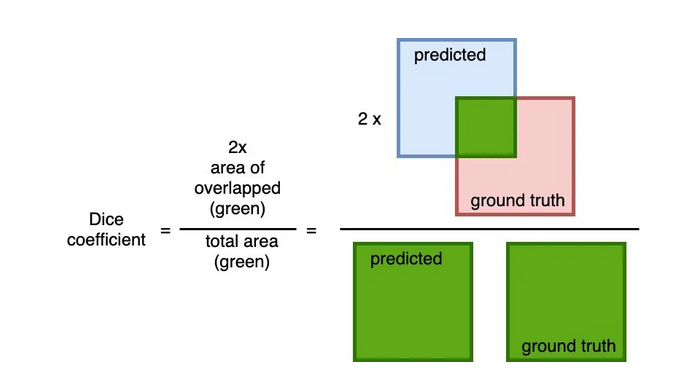
\includegraphics[width = 4.8in]{../images/DSC.png}}
    \caption{Example explaining Dice coefficient}
    \label{fig:DSC_EX}
\end{figure}

This coefficient is not very different in form from the Jaccard index (IOU). In fact, both are equivalent in the sense that given a value for the Sørensen–Dice coefficient $S$ , one can calculate the respective Jaccard index value $J$  and vice versa, using the equations : 
\begin{equation}
    J = \frac{DSC}{( 2 − DSC )}
\end{equation}

and 

\begin{equation}
    DSC = \frac{2 J  }{( 1 + J )}
\end{equation}

The function ranges between zero and one, like Jaccard. the corresponding loss function:
\begin{equation}
    DSC\_LOSS = 1 - \frac{2 TP}{2 TP + FN + FP}
\end{equation}

\subsection{Tversky}
\hspace{\parindent}
The Tversky index, named after Amos Tversky, is an asymmetric similarity measure on sets that compares a variant to a prototype. The Tversky index can be seen as a generalization of the Sørensen–Dice coefficient and the Dice coefficient (aka Jaccard index).
For sets X and Y the Tversky index is a number between 0 and 1 given by :
\begin{equation}
    S(X, Y) = \frac{| X \cap Y |}{| X \cap Y | + \alpha|X  ∖ Y| + \beta | Y  ∖  X|}
\end{equation}
Here, $X ∖ Y$ denotes the relative complement of Y in X. 
Further, $\alpha , \beta \geq 0$  are parameters of the Tversky index. Setting $\alpha = \beta = 1$ produces the Jaccard coefficient; setting $\alpha = \beta = 0.5$  produces the Sørensen–Dice coefficient. 

The function ranges between zero and one, the corresponding loss function:

\begin{equation}
    S\_LOSS(X, Y) =  1 - \frac{| X \cap Y |}{| X \cap Y | + \alpha|X  ∖ Y| + \beta | Y  ∖  X|}
\end{equation}

\subsection{Cross-entropy}
\hspace{\parindent}
Cross-entropy loss, or log loss, measures the performance of a classification model whose output is a probability value between 0 and 1. Cross-entropy loss increases as the predicted probability diverges from the actual label. So predicting a probability of .012 when the actual observation label is 1 would be bad and result in a high loss value. A perfect model would have a log loss of 0.

The cross-entropy for a single example in a binary classification task can be stated by unrolling the sum operation as follows:

\begin{equation}
    H(X, Y) = - (X(class0) * log(Y(class0)) + X(class1) * log(Y(class1)))
\end{equation}

\subsection{Mean Squared Error}
\hspace{\parindent}
Mean squared error (MSE) is simply defined as the average of squared differences between the predicted output and the true output. Squared error is commonly used because it is agnostic to whether the prediction was too high or too low, it just reports that the prediction was incorrect.

This is the Mean Squared Error formula:

\begin{equation}
    MSE = \frac{1}{n} \sum_{i=1}^{n} (Y_{i} - \hat{Y}_{i})^{2}
\end{equation}

We used this loss function in both our DO-U-Net and DO-SegNet models for predicting red and white blood cells.\

There is however a slight problem, the Mean Squared Error has the disadvantage of heavily weighting outliers.[11] This is a result of the squaring of each term, which effectively weights large errors more heavily than small ones.

\section{Conclusion}
\vspace{0.2in}
\hspace{\parindent}
In this chapter we presented the components of our method from segmentation models and their metrics, loss functions and data augmentation. We also explained the counting methods that we are using in our solution.

\newpage
